The Control Unit layer is responsible for processing input data, managing system logic, and generating output signals. The Control Unit includes sound settings, user settings, and a sound multiplexer.

\subsection{Layer Hardware}
The Control Unit layer uses a Raspberry Pi 4 as its primary hardware component.

\subsection{Layer Operating System}
This layer uses Raspberry Pi OS

\subsection{Layer Software Dependencies}
N/A

\subsection{Sound Setting}
The Sound Settings subsystem receives digital signals from the UserSettings and the Sound Settings subsystem is responsible for managing and applying the sound settings based on user input.

\begin{figure}[h!]
	\centering
 	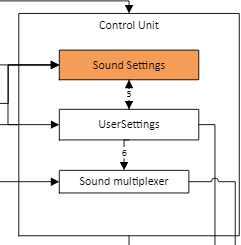
\includegraphics[width=0.60\textwidth]{architectural design specification latex/dds/detailed design specification latex/images/SoundSettings.png}
 \caption{Example subsystem description diagram}
\end{figure}

\subsubsection{Subsystem Hardware}
N/A

\subsubsection{Subsystem Operating System}
Raspberry pi OS    

\subsubsection{Subsystem Software Dependencies}
 N/A

\subsubsection{Subsystem Programming Languages}
 The subsystem uses Python for managing sound settings

\subsubsection{Subsystem Data Structures}
N/A

\subsubsection{Subsystem Data Processing}
N/A

\subsection{USerSetting}
The UserSettings subsystem is connected to the Sound Settings and the Sound Multiplexer subsystem

\begin{figure}[h!]
	\centering
 	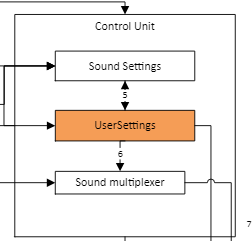
\includegraphics[width=0.60\textwidth]{architectural design specification latex/dds/detailed design specification latex/images/UserSettings.png}
 \caption{Example subsystem description diagram}
\end{figure}


\subsubsection{Subsystem Hardware}
N/A

\subsubsection{Subsystem Operating System}
Raspberry pi OS 

 \subsubsection{Subsystem Programming Languages}
 The subsystem uses Python for managing user settings

\subsubsection{Subsystem Data Structures}
N/A

\subsubsection{Subsystem Data Processing}
N/A

\subsection{Sound multiplexer.}
The Sound Multiplexer subsystem is connected to the Sound Settings subsystem and the Output Layer

\begin{figure}[h!]
	\centering
 	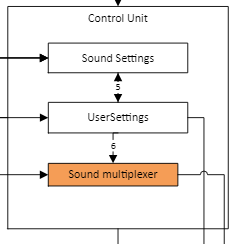
\includegraphics[width=0.60\textwidth]{architectural design specification latex/dds/detailed design specification latex/images/Soundmultiplex.png}
 \caption{Example subsystem description diagram}
\end{figure}

\subsubsection{Subsystem Hardware}
N/A

\subsubsection{Subsystem Operating System}
Raspberry pi OS

 \subsubsection{Subsystem Programming Languages}
 The subsystem uses Python for managing Sound multiplexer
